\chapter{使用介绍}
\section{配置编译环境}

在这一章中,手册使用的操作系统为Ubuntu 18.04.5 LTS,编译交叉工具链为arm-2010q1。其它版本的操作系统和编译器可以自行测试。

(1)第一步,将编译器加入系统环境变量。在终端输入
\begin{lstlisting}
 gedit /etc/profile   
\end{lstlisting}

在打开的文件最后输入
\begin{lstlisting}
 PATH=xxx/arm-2010q1/bin:\$PATH  
\end{lstlisting}

其中“xxx”为交叉编译链文件所在路径。然后保存文件,在终端输入
\begin{lstlisting}
 source etc/profile
\end{lstlisting}

更新环境变量。最后在终端输入
\begin{lstlisting}
 arm-none-eabi-gcc -v
\end{lstlisting}

查看版本号,确定交叉编译工具是否安装成功。

(2)第二步,修改编译所需的编译器。修改aCoral根目录下的Makefile文件中的交叉编译路径CROSS\_COMPILE 为
\begin{lstlisting}
 xxx/arm-2010q1/bin/arm-none-eabi-
\end{lstlisting}

其中“xxx”为交叉编译链文件所在路径。

(3)第三步,编译。进入aCoral根目录,在终端输入
\begin{lstlisting}
 make
\end{lstlisting}

等待编译完成之后,就会得到我们要下载的aCoral镜像文件acoral.bin以及一些辅助文件。

\section{aCoral内核下载}

在得到acoral.bin镜像文件后,我们就可以将其下载到开发板上了。
理论上我们可以直接把acoral.bin烧写到开发板的nor flash或者nand flash上启动,aCoral可以自我引导,即将自己复制到sdram内存中执行。
但是这有一个问题,烧写到nor flash或者nand flash的速度是很慢的,如果我们每次在修改aCoral的源码后,
直接烧写到开发上进行调试,就会浪费大量时间在等待烧写完成上。

对于这个问题,我们有一种解决方案,就是在nor flash或者nand flash中烧写一个bootloader,每次修改源码编译得到新镜像后,
使用bootloader,将新编译得到的内核镜像直接复制到sdram中执行,这样就可以节省很多时间。
本手册中,bootloader我们使用友善之臂开发的supervivi。关于supervivi如何烧写进flash,请自行在网上查找资料。
这里我们默认已经在nor flash中烧写好了supervivi。接下来就可以正式开始下载aCoral。

(1)第一步,接线。依次从左到右插上USB下载线、串口线、电源线,如图\ref{接线示意图}所示。
\begin{figure}[H]
	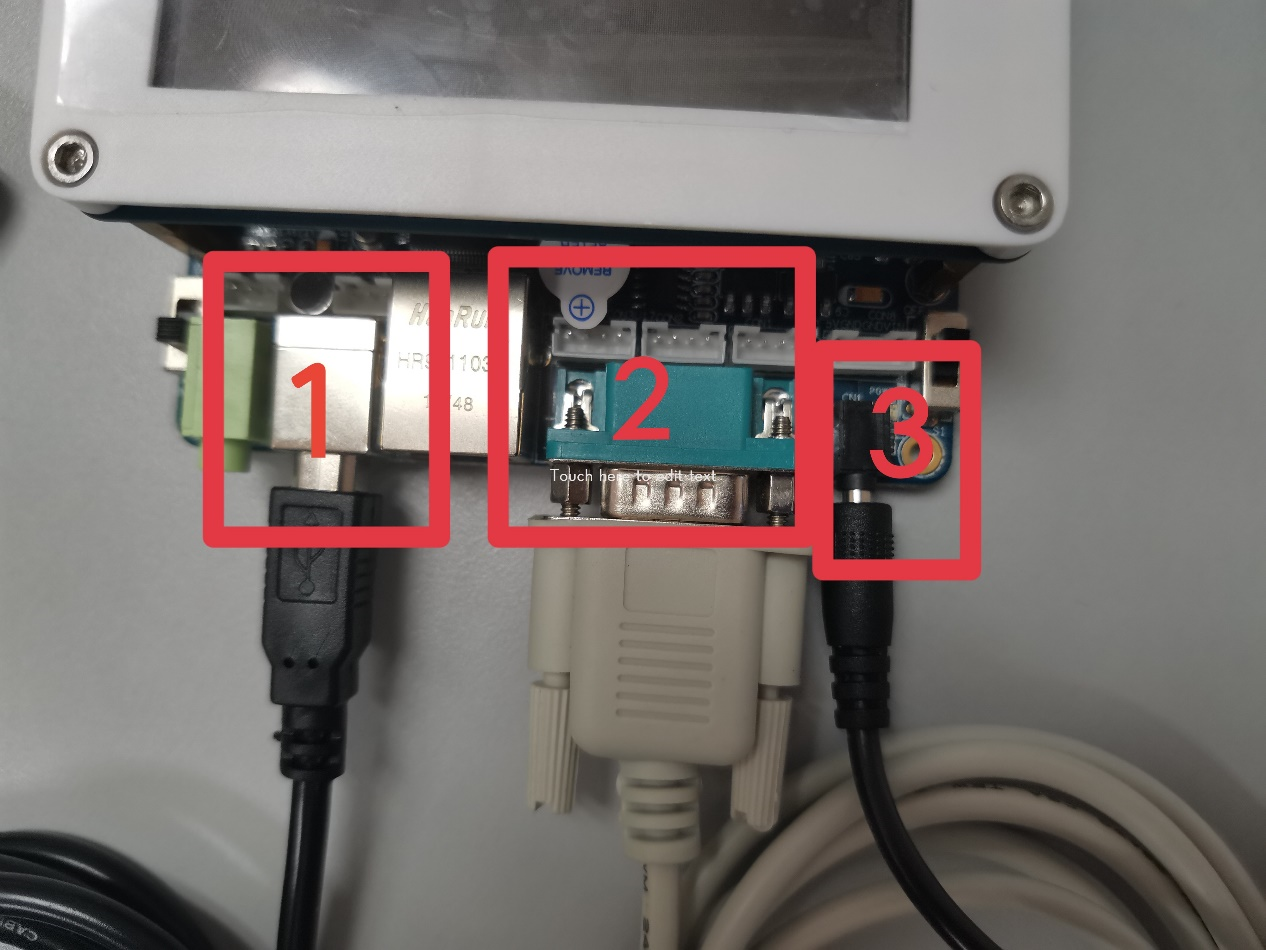
\includegraphics[width=\textwidth]{接线示意图.png}
	\caption{接线示意图}
	\label{接线示意图}
\end{figure}

USB下载线和串口线另一端USB接口自然是插到电脑上。其中USB下载线用于将镜像下载到sdram中,串口线用于在开发板和PC之间传递字符信息,
比如命令行命令就是由串口线传到开发板上,执行结果再由串口回显到PC上。大家电脑上肯定没有串口了,所以需要一个USB转串口驱动(PL2303芯片)。
如何在Ubuntu下安装PL2303驱动,参考 \href{https://blog.csdn.net/qq_34562093/article/details/75059251}{\underline{ubuntu安装USB转串口驱动(PL2303)}}

(2)第二步,安装mimicom串口工具,并能够正确识别插上的USB转串口。具体自行查阅资料。

(3)第三步,将开发板左下角的开关向下拨到nor,如图\ref{nor开关}所示。
\begin{figure}[H]
	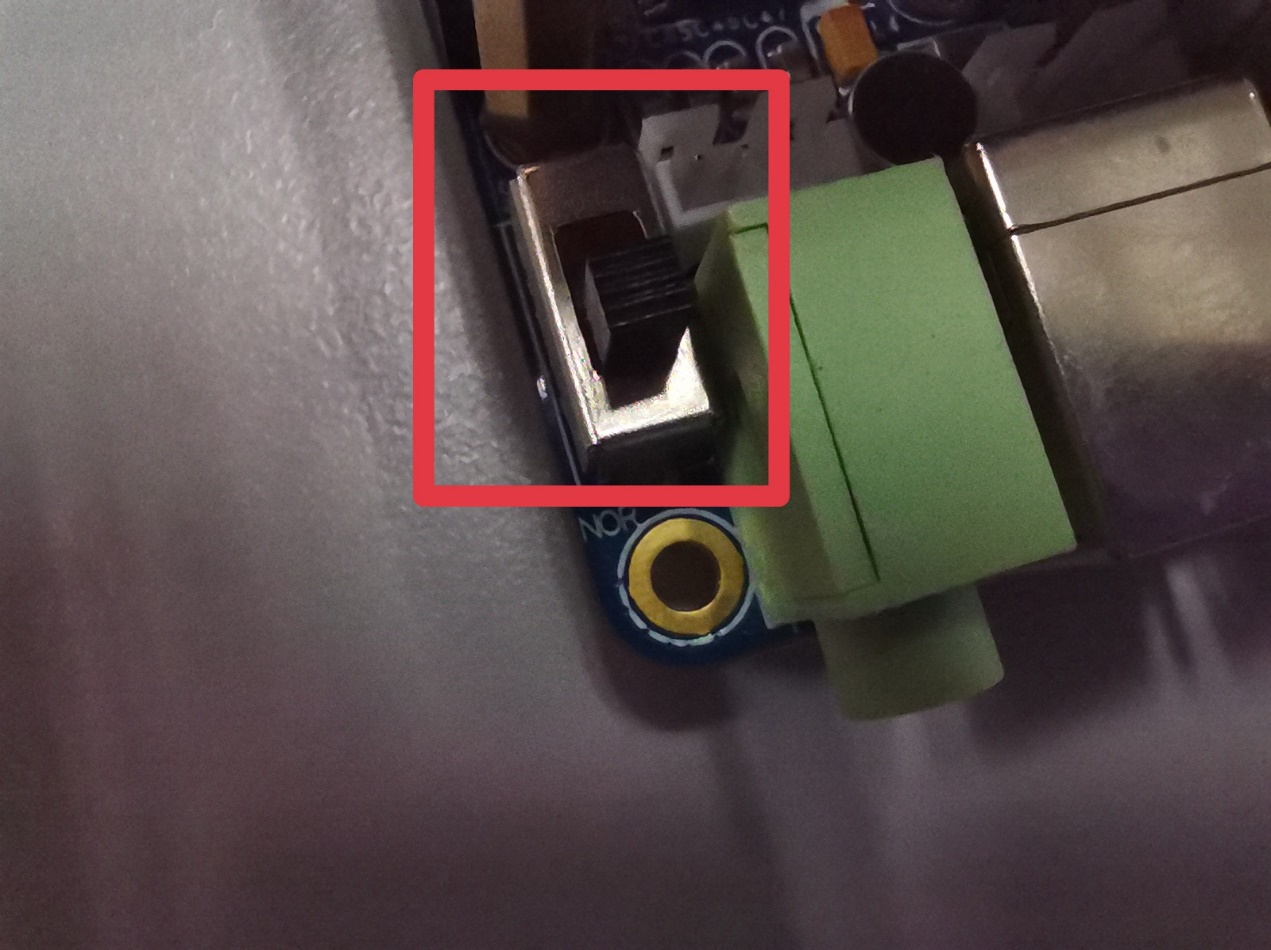
\includegraphics[width=\textwidth]{nor开关.png}
	\caption{nor开关}
	\label{nor开关}
\end{figure}

(4)第四步,编译aCoral根目录下的dnw.c文件。这里我们已经提前编译好了dnw,直接使用即可。dnw就是USB下载线的驱动。

(5)运行minicom,连接好串口,打开mini2440的电源开关,你将看到如下界面:

输入d,看到如下界面:

运行dnw,下载acoral.bin,如图:

如果一切顺利,你将在minicom看到如图所示的界面,表示aCoral已经在内存sdram中运行起来了,吗,minicom上显示出"aCoral:>",这就是aCoral的shell。

大家可以在中输入help命令,看看aCoral现在支持的指令。
至此,aCoral的下载完成,之后如果又重新编译了新的镜像,都可以按照这个步骤来。
需要注意的是,这种使用bootloader直接往sdram下载的镜像,关机之后没了,需要重新下载。